\documentclass[a4paper,10pt,titlepage]{scrbook}
\usepackage{color}
\usepackage{mathptmx}
\usepackage{amssymb,amsmath} % math symbols
\usepackage{amstext}
\usepackage{tikz} % draw graphs and many more
\usepackage{color}
\usepackage{xspace}
\usepackage{hyperref}
\usepackage{verbatim}
\usepackage{enumerate}
\usepackage{float}
\floatstyle{boxed} 
\restylefloat{figure}

\thispagestyle{empty}

\definecolor{ratBordeaux1}{HTML}{A11035}
\definecolor{ratBordeaux2}{HTML}{B65256}
\definecolor{ratBordeaux3}{HTML}{CD8B87}
\definecolor{ratRed1}{HTML}{CC071E}
\definecolor{ratRed2}{HTML}{D85C41}
\definecolor{ratRed3}{HTML}{E69679}
\definecolor{ratLila}{HTML}{7A6FAC}
\definecolor{ratGreen}{HTML}{57AB27}
\definecolor{ratLila2}{HTML}{9B91C1}
\definecolor{ratGreen2}{HTML}{8DC060}
\definecolor{ratMagenta}{HTML}{E30066}
\definecolor{ratViolett3}{HTML}{D2C0CD}
\definecolor{ratViolett}{HTML}{7A6FAC}
\definecolor{ratOrange}{HTML}{F6A800}
\definecolor{ratYellow}{HTML}{FFED00}
\definecolor{ratTurquoise}{HTML}{00B1B7}
\definecolor{ratLimeGreen}{HTML}{BDCD00}
\definecolor{ratLimeGreen}{HTML}{BDCD00}
\definecolor{ratGray}{HTML}{9C9E9F}

\begin{document}
\begin{center}
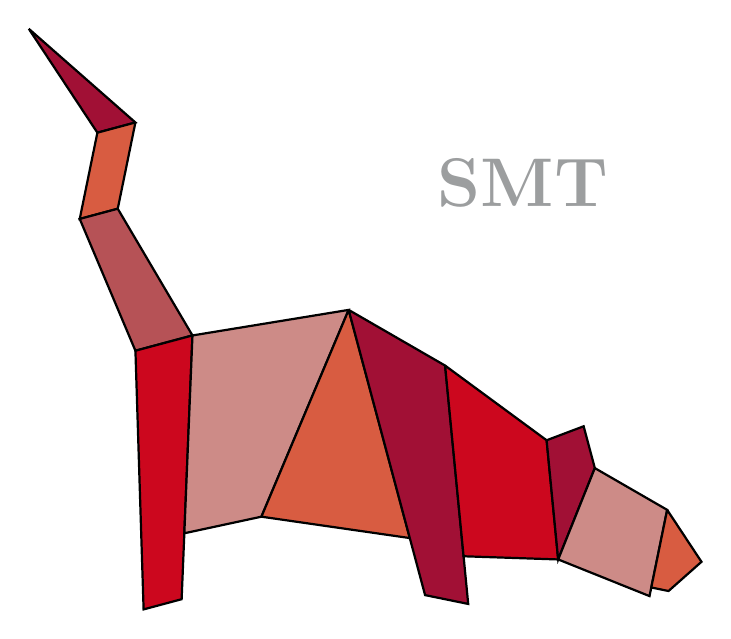
\begin{tikzpicture}[scale=.5,rotate=285]
    \node (smt) at (7,12) {\color{ratGray}\fontsize{120}{100} \selectfont \textbf{SMT}};
    \fill [draw=black, thick, fill=ratBordeaux1] (0,1) -- (3,3) -- (3,2) -- (0,1);
    \fill [draw=black, thick, fill=ratRed2] (3,3) -- (5,2) -- (5,1) -- (3,2) -- (3,3);
    \fill [draw=black, thick, fill=ratBordeaux2] (5,2) -- (8.6,3) -- (8.6,1.5) -- (5,1) -- (5,2);
    \fill [draw=black, thick, fill=ratRed1] (8.6,3) -- (15,1) -- (15,0) -- (8.6,1.5) -- (8.6,3);
    \fill [draw=black, thick, fill=ratBordeaux3] (8.6,3) -- (13.4,1.5) -- (13.5,3.5) -- (9,7) -- (8.6,3);
    \fill [draw=black, thick, fill=ratRed2] (9,7) -- (15,7) -- (13.5,3.5) -- (9,7);
    \fill [draw=black, thick, fill=ratBordeaux1] (9,7) -- (16.5,7) -- (17,8) -- (11,9) -- (9,7);
    \fill [draw=black, thick, fill=ratRed1] (11,9) -- (15.8,8.2) -- (16.5,10.5) -- (13.5,11) -- (11,9);
    \fill [draw=black, thick, fill=ratBordeaux1] (13.5,11) -- (13.4,12) -- (14.5,12) -- (16.5,10.5) -- (13.5,11);
    \fill [draw=black, thick, fill=ratBordeaux3] (14.5,12) -- (16,13.5) -- (18,12.5) -- (16.5,10.5) -- (14.5,12);
    \fill [draw=black, thick, fill=ratRed2] (16,13.5) -- (17.5,14) -- (18,13) -- (17.8,12.6) -- (16,13.5);
\end{tikzpicture}
\end{center}
\end{document}
